% Document class `report-template` accepts either project-plan or final-report option in
% []. This will change the title page as necessary.
\documentclass[project-plan]{report-template}
%\documentclass[final-report]{report-template}

% Packages I use in my report.
\usepackage{graphicx}
\usepackage{amsmath}
\usepackage{blindtext}

% Directory where I saved my figures.
\graphicspath{{./figures/}}

% Metadata used for the title page
\university{Imperial College London}
\department{Department of Earth Science and Engineering}
\course{MSc in Environmental Data Science and Machine Learning}
\title{Noise reduction in seismic images, investigating deep learning from natural image models}
\author{Robert Smith}
\email{robert-edward-duncan.smith23@imperial.ac.uk}
\githubusername{edsml-rs4623}
\supervisors{James Lowell, Geoteric\\
             Prof. Rebecca Bell}
\repository{https://github.com/edsml-rs4623/IRP-2024}

\begin{document}

\maketitlepage  % generate title page

% Abstract
\section*{Abstract}
\blindtext  % outputs some dummy text

\newpage
\tableofcontents
\newpage

% Introduction section
\section{Introduction}
High quality seismic images are crucial for understanding underground geological structures. They facilitate qualitative and quantitative interpretation and enable further analysis such as automated feature recognition.

Owing to the complex nature of the Earth's subsurface and the seismic image construction process noise inevitably contaminates the data and can significantly affect its quality. This noise can be caused by many factors during both the reflection data acquisition process, for example from environmental noise, as well as during processing, such as migration. 

Various factors contribute to seismic noise, but they can be classified into two broad types: coherent noise and random noise. Coherent noise is signal dependent that shows consistent phase from trace to trace, examples are include ground roll and multiples. Random noise that is uncorrelated from trace to trace often caused by disturbances in the sub-surface environment. Effective noise attenuation removes noise whilst preserving the signals from the seismic data improving the signal-to-noise ratio (SNR).

There are a multitude of traditional methods for attenuating noise that have been used. Some of these methods include; filter-based strategies, such as mean filtering~\cite{Liu20062d} or f-x de-convolution ~\cite{hornbostel1991spatial}; spare transformation-based strategies, such as using Fourier transforms ~\cite{alsdorf1997noise} or wavelet transform ~\cite{Albert2009wavelet}; and modal decomposition techniques, such as empirical mode decomposition ~\cite{bekara2009random} and singular value decomposition ~\cite{bekara2007local}. These methods have differing drawbacks such as they are not adaptive, applying consistently across the data, and they often rely on expert experience for manual parameter selection.

In recent years there has been a vast amount of research and many advances in the application of deep learning to tasks for natural image datasets, including on models to denoise and improve image quality. The drawbacks of traditional methods, combined with these advances and available computational power, have led to the application of deep neural network models for seismic denoising. 

Whilst various application of deep learning frameworks to seismic data have been explored, there has been little in the way of utilising the more current architectures, and their trained models, proven effective on natural images. Given the ability for modern deep neural networks to effectively extract multi-scale  features for natural images and produce models that can generalise across domains. The challenge then is to to explore the progress in deep learning frameworks for natural datasets, and their applicability to seismic data.  Investigate and evaluating the effectiveness of different transfer learning approaches and training strategies, utilising Geoteric's in-house synthetic data model to produce training data.

Improving the noise removal process is a significant area for research as it enables more accurate imaging and thus improved interpretation of the geological structures. This work seeks to further develop the area of seismic image de-noising using deep learning, and contribute towards the commercial development of denoising/restoration products. High quality seismic data also facilitate down-stream applications such as for identifying appropriate sites Carbon Capture, Utilisation and Storage.

\subsection{Literature review}
[As noise removal is a highly ill-posed problem. Deep learning networks implicitly learning by capturing natural image statistics from large data sets]
The use of neural networks, specifically convolutional neural networks (CNNs), have led the advancements in learning models for Image restoration and denoising over recent years. Many state of the art networks for denoising use CNNs as they are able to learn spatial hierarchies of patterns and to learn generalised image priors.

The use of residual blocks in CNNs ~\cite{he2015DeepRL} allowed gradients to flow through the block helping to address the issue of vanishing gradients facilitating the use of much deeper networks. In image restoration tasks where the original mapping is closer to an identity mapping, the residual mapping will be much easier to optimise and can improve performance. Residual blocks were then implemented in the influential denoising convolutional neural network (DcCNN) ~\cite{zhang2017beyond}, which lead to significantly increased denoising performance than traditional Gaussian denoisers. 

Some CNN models were then developed to be fast and flexible in their application, ~\cite{zhang2018ffdnet} used sub-sampling and shallower networks as well as a noise level map input. However, these non-blind denoisers require knowledge of the image noise, which can reduce performance for real images where spatially variant noise is hard to estimate.  

In order to create models that generalise well, blind models incorporated a noise model, and contained a sub-network to learn the noise and another non-blind denoiser ~\cite{Guo2019Cbdnet}. The model generalised better and when trained on synthetic and real noisy images they improved performance against benchmarks. However these models are dependent on developing a good noise model and having real noisy data with ground-truths, both of which can be challenging.

In order to allow the model to selectively focus on the important parts of the input data various attention mechanisms have been implemented into computer vision models ~\cite{wang2017residual} ~\cite{hu2018senet}~\cite{woo2018cbam}~\cite{wang2020eca}~\cite{hou2021coordinate}. Incorporating simple feature attention has improved the performance of Denoising networks ~\cite{anwar2019real}. Combining attention mechanisms, for example to enhance the spatial and channel representation of the model, have be shown to improve networks ~\cite{cai2023cbamdncnn}.

Recently more complex architectures that combine attention with capturing multi-scale resolution, aiming to capture both high resolution spatially precise representations along with maintaining low resolution representations with contextual information, have achieved state of the art results.~\cite{zamir2020MIRNet}. Multi-stage models based on the ides of progressively learning to capture contextual and spatial features~\cite{zamir2021MPRNet} have also achieved compelling results, however these networks are very complex and are more computationally expensive.

Transformer based image restoration models, leveraging self attention mechanisms to capture long range pixel interactions effectively, have also produced similar state of the art results for denosing~\cite{zamir2021restormer}~\cite{wang2022uformer}. Transformer networks computational requirements can increase drastically with increase in image resolution, a potential fix has been to incorporate  self-attention within local regions using Swin transformer design ~\cite{wang2022uformer}. Further designs have improved the context aggregation capability of these networks~\cite{zamir2021restormer}.

\subsection{training schemes}
Supervised deep learning models can perform well on denoising then but require a realistic noisy and clean image pairs to learn mappings, and a significant amount of realistic data to be able to generalise. Self supervised learning strategies can then help resolve some of these challenges as they don't require clean images for training. Noise2Noise~\cite{} pioneered this approach by denoising images using solely noisy images to train and producing performance similar to existing using clean labels. Many other self-supervised strategies have been developed including, Noise2void~\cite{}, Noise2self.

difficulties in the application of deep learning is
Self-supervised 
Due to the  lack of real training data for seismic models and reliance on synthetic data. 

Perform well on random noise but not coherent - 

% Figure
\begin{figure}[htb]
    \begin{center}
        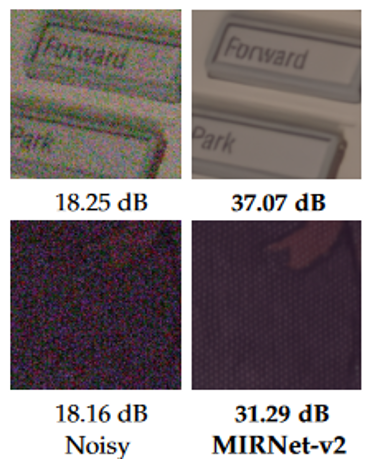
\includegraphics[width=0.4\textwidth]{latex/figures/noise_removal_ex.png}
    \end{center}
    \caption{\label{fig:experiment} Example denoising results from CNN network.}
\end{figure}

\subsection{Objectives}
The project aims to investigate using established and proven model architectures alongside Geoteric's in-house synthetic seismic generation model. Specifically, learning from natural image denoising by leveraging models and techniques that have proved successful.
The ultimate objective is to developing a deep learning seismic denoising model that effectively removes noise, and improves the performance of their existing methods.  Potentially expanding to 3D seismic sections if model performance justifies and time allows.


\section{Methodology}
As per the project brief there has been a significant amount of research and advances in the application of Deep learning to natural image datasets, including on models to denoise and improve image quality.

loss functions and training schemes

I will look to use a deep convolutional neural network with residual attention mechanism
- Other models
- Synthetic data
- Building own model specific to seismic


\section{Expected Outcomes}
The project looks to give clarity on the feasibility of 

\section{Future work}
\subsection{Progress to date}
In this work, we wrote a simulation package for calculating the position of a particle in vertical motion as shown in Fig.~\ref{fig:experiment}. We compute the position $y(t)$ at time $t$ using:

\section{Future work}

% References
\bibliographystyle{plain}
\bibliography{references}  % BibTeX references are saved in references.bib

\end{document}          
